\documentclass[a4paper]{article}
\usepackage{fullpage}
\usepackage{lipsum}
\usepackage[textsize=\tiny]{todonotes}
\usepackage{graphicx} % Required for inserting images
\usepackage[sort]{natbib}
\usepackage{amsthm, amsmath, amssymb, mathtools}
\usepackage{bm}
\usepackage{mathrsfs, eufrak}
\usepackage{hyperref}
\usepackage[capitalize, sort, noabbrev]{cleveref}
\usepackage[shortlabels]{enumitem}
% \usepackage[bbgreekl]{mathbbol}
\usepackage{xcolor}

\hypersetup{
    colorlinks,
   linkcolor={red!50!black},
   citecolor={red!50!black},
   urlcolor={red!50!black}
}

\theoremstyle{definition}
\newtheorem{definition}{Definition}
\newtheorem{assumption}{Assumption}

\theoremstyle{remark}
\newtheorem{remark}{Remark}

\theoremstyle{plain}
\newtheorem{theorem}{Theorem}
\newtheorem{property}{Property}
\newtheorem{proposition}{Proposition}
\newtheorem{lemma}{Lemma}
\newtheorem{corollary}{Corollary}

\bibliographystyle{apalike}

\title{The Value Equivalence Principle: A Summary}
\author{Alireza Kazemipour}
\date{\today}

\newcommand{\bA}{\mathbf{A}}
\newcommand{\bO}{\mathbf{O}}
\newcommand{\bS}{\mathbf{S}}
\newcommand{\bE}{\mathbf{E}}
\newcommand{\bP}{\mathbf{P}}
\newcommand{\cR}{\mathcal{R}}
\newcommand{\cT}{\mathcal{T}}
\newcommand{\sF}{\mathscr{F}}
\newcommand{\bG}{\mathbf{G}}
\newcommand{\cN}{\mathcal{N}}
\newcommand{\cH}{\mathcal{H}}
\newcommand{\bM}{\mathbf{M}}
\newcommand{\bV}{\mathbf{V}}
\newcommand{\bW}{\mathbf{W}}
\newcommand{\bX}{\mathbf{X}}
\newcommand{\bY}{\mathbf{Y}}
\newcommand{\bZ}{\mathbf{Z}}
\newcommand{\bPi}{\mathbf{\Pi}}
\newcommand{\bDelta}{\mathbf{\Delta}}
\newcommand{\fB}{\mathfrak{B}}
\newcommand{\C}{\mathbb{C}}
\newcommand{\R}{\mathbb{R}}
\newcommand{\K}{\mathbb{K}}
\newcommand{\N}{\mathbb{N}}
\newcommand{\II}{\mathbb{I}}
\renewcommand{\P}{\mathbb{P}}
\newcommand{\E}{\mathbb{E}}
\DeclareMathOperator*{\argmax}{arg\,max}
\renewcommand{\dim}{\textsf{dim}}
\DeclareMathOperator{\Hdim}{\textsf{H-dim}}
\DeclareMathOperator*{\argmin}{arg\,min}

\newcommand{\AK}[1]{\textcolor{teal}{(\textbf{AK}: {#1})}}

\begin{document}

\maketitle

\begin{abstract}
    As of \date{\today}: In this document I intend to summarize, highlight my gaps in understanding, and my gut feelings around future directions regarding: Value-aware model learning (VAML)~\citep{farahmand2017value}, the value equivalence (VE) principle~\citep{grimm2020value}, proper value equivalence (PVE)~\citep{grimm2021proper}, and model equivalence principle for risk-sensitive reinforcement learning~\citep{kastner2023distributional}. Especially, the first and the last references are pretty precise, so I should be able to understand them.
\end{abstract}

\section*{Notation guide}
\begin{itemize}
    \item Bold letters denote sets.
    \item Calligraphic letters denote distributions.
    \item Capital letters denote subsets (note that random variables are subsets).
    \item Lower case letter denote elements that belong to a set.
\end{itemize}
    
\section{Introduction}
\label{sec:intro}
Let our MDP be the tuple $\left \langle \bS, \bA, p^*, r^*, \gamma \right \rangle$, where $p^*$ is the transition kernel and $r^*: \bS \times \bA \to \fB(\R)$ is the immediate expected reward function which we assume is know to the agent in advance. The goal in model-based reinforcement learning (MBRL) has traditionally been learning an estimate $\hat{p}$ of $p^*$, and then using $\hat{p}$ for planning to produce an optimal policy. Estimating $p^*$ by $\hat{p}$ is problem of conditional probability estimation and the goal is to make $\hat{p}$ as \emph{close} as possible to $p^*$. 

One approach to estimate $p^*$ is by maximum-likelihood estimation (MLE) method. The reason MLE is an appropriate approach is because of its relation to KL divergence. We know that for two distributions $p_1$, and $p_2$, the KL divergence $\textsf{KL}(p_1 ||p_2)$ is zero if and only of $p_1 = p_2$ almost surely. So, now we show that maximizing the likelihood, minimizes the KL divergence which is the goal. Suppose $p_1$ is the distribution we want to estimate with the true parameter $\theta^*$, and $p_2$ is our estimate. We want to find parameters $\theta_{\mathsf{min}}$ such that
\begin{align*}
    \theta_{\mathsf{min}} &= \argmin_\theta \mathsf{KL}(p_1(\cdot; \theta^*) || p_2(\cdot; \theta)) \\
    & = \argmin_\theta \E_{x \sim p_1(\cdot; \theta^*)}\left[\log \frac{p_1(x; \theta^*)}{p_2(x; \theta)}\right] \\
    & = \argmin_\theta \E_{x \sim p_1(\cdot; \theta^*)}\left[\log p_1(x; \theta^*) -\log p_2(x; \theta)\right] \\
    & = \argmin_\theta \E_{x \sim p_1(\cdot; \theta^*)}\left[-\log p_2(x; \theta)\right] \tag{$\log p_1(x; \theta^*)$ doesn't affect the argument of minima} \\
    & = \argmax_\theta \E_{x \sim p_1(\cdot; \theta^*)}\left[\log p_2(x; \theta)\right] \\
    & = \argmax_\theta \E_{x \sim p_1(\cdot; \theta^*)}\left[\log p_2(x; \theta)\right] \\
    & = \argmax_\theta \sum_i^n p_1(x_i; \theta^*)\log p_2(x_i; \theta) \tag{If we have a dataset of size $n$} \\
    & = \argmax_\theta \log \Pi_i^n p_2(x_i; \theta)\tag{$p_1(x_i; \theta^*)$ doesn't affect the argument of maxima} \\
    & = \argmax_\theta \Pi_i^n p_2(x_i; \theta) \tag{MLE definition}.
\end{align*}
Hence, MLE is a viable option to estimate $p^*$ by $\hat{p}$. The MLE approach has been the dominant strategy in MBRL traditionally. Making $\hat{p}$ close to $p^*$ through MLE in MBRL is also justified by the fact that the resulting loss because of the mismatch of $\hat{p}$ and $p^*$ in estimating action value of a policy $\pi$ for state-action $(s, a) \in \bS \times \bA$ is upper bounded as the following:
\begin{align*}
    \ell\left(\hat{p}, p^*; v_\pi\right)(s, a) & = \left \lvert \left[p^*(\cdot \mid s, a) - \hat{p}(\cdot \mid s, a) \right]v_\pi(\cdot)\right\rvert \\ 
    & = \left\langle p^*(\cdot \mid s, a) - \hat{p}(\cdot \mid s, a), v_\pi\right\rangle \\
    & \leq \left\lVert p^*(\cdot \mid s, a) - \hat{p}(\cdot \mid s, a)\right\rVert_1 \cdot \lVert v_\pi \rVert_\infty \tag{H{ö}lder's inequality} \\
    & \leq \sqrt{2\mathsf{KL}(p^*||\hat{p})} \cdot \lVert v_\pi \rVert_\infty. \tag{Pinsker's inequality}
\end{align*}
Since MLE minimizes the KL divergence, the above display justifies the use of MLE. The transition kernel follows the multinomial distribution and the MLE for this distribution prescribes that if the state-action $(s, a)$ is visited $N(s, a)$ times and the next state visited after the $i$th visit is $S_i$ then
\begin{equation*}
    \hat{p}\left(s' \middle\vert s, a\right) = \frac{1}{N(s, a)}\sum_{i=1}^{N(s, a)}\II\left\{S'_i = s'\right\},\quad  \forall s' \in \bS.
\end{equation*}
%
Nonetheless, the task-agnostic model learning is wasteful. There is no need to learn an accurate model for parts of the environment that are irrelevant to the task hand. For example, for a cooking-assistant robot the dynamics of the elevator inside the building is not of interest. Hence, model learning should be tailored toward the task at hand. This argument is at the core of alternative perspectives that will come in the following sections.

\section{VAML}
\citet{farahmand2017value} directly considers $\ell\left(\hat{p}, p^*; v_\pi\right)$. Instead of the pointwise distance, they consider a weighted loss where the weighting $\nu \in \bDelta(\bS \times \bA)$\footnote{$\bDelta(\bX)$ represents the set of probability distributions over the set $\bX$.} is probability distribution that puts weights on important state-actions. Second, instead of the $L_1(\nu)$-norm loss, they consider the $L_2(\nu)$-norm. Third, they consider the the distance under the worse value function in their function class $\bV$.
\begin{equation}
    \label{eq:vaml-loss}
    \ell^2_2\left(\hat{p}, p^*\right) = \int d\nu(x, a) \sup_{v \in \bV} \left \lvert \int \left[p^*\left(ds' \middle\vert s, a\right) - \hat{p}\left(ds' \middle\vert s, a\right)\right]v\left(s'\right) \right \rvert^2
\end{equation}
Similar to what we showed in \cref{sec:intro}, we can bound the right-hand side of \cref{eq:vaml-loss} as follows:
\begin{equation}
    \label{eq:ub-vaml}
    \sup_{v \in \bV} \left \lvert \int \left[p^*\left(ds' \middle\vert s, a\right) - \hat{p}\left(ds' \middle\vert s, a\right)\right]v\left(s'\right) \right \rvert \leq 
     \left \lVert p^*(\cdot \mid s, a) - \hat{p}(\cdot \mid s, a) \right \rVert_1 \sup_{v \in \bV}\lVert v \rVert_\infty.
\end{equation}
But, the right-hand side of \cref{eq:ub-vaml} is quite loose. Specifically, $\sup_{v \in \bV}\lVert v \rVert_\infty$ can be very large while the on the left-hand side the value of $\sup$ is also controlled by the mismatch between distribution. Hence, VAML aims to optimize the left-hand side of \cref{eq:ub-vaml} through \cref{eq:vaml-loss} by first gathering data using some procedure, minimize the loss and handing off the learned transition kernel to the planner. Then, VAML provides an upper bound on \cref{eq:vaml-loss}. In order to state the upper bound, it is useful to revisit some concepts from the supervised learning literature.
%
\begin{definition}[{\normalfont\citet{gyorfi2002distribution}[Definition 9.3]}]
    Let $\epsilon > 0$, let $\bG$ be a set of function $\R^d \to \R$, $1 \leq p \leq \infty$, and let $\nu$ be a probability measure on $\R^d$. For a function $f: \R^d \to \R$ set
    \begin{equation*}
        \lVert f \rVert_{L_p(\nu)} \coloneq \left[\int |f(z)|^pd\nu\right]^\frac{1}{p}.
    \end{equation*}
    \begin{enumerate}[label=(\alph*)]
        \item Every finite collection of functions $g_1, \dots, g_N: \R^d \to \R$ with the property that for every $g \in \bG$ there is a $j = j(g) \in \{1, \dots, N\}$ such that 
        \begin{equation*}
            \left\lVert g - g_j \right\rVert_{L_p(\nu)} < \epsilon
        \end{equation*}
        is called and $\epsilon-$cover of $\bG$ with respect to $\left\lVert \cdot \right\rVert_{L_p(\nu)}$.
        
        \item Let $\cN\left(\epsilon, \bG, \left\lVert \cdot \right\rVert_{L_p(\nu)} \right)$ be the size of the smallest $\epsilon$-cover of $\bG$ w.r.t $\left\lVert \cdot \right\rVert_{L_p(\nu)}$. Take $\cN\left(\epsilon, \bG, \left\lVert \cdot \right\rVert_{L_p(\nu)} \right) = \infty$ if no finite $\epsilon$-cover exits. Then, $\cN\left(\epsilon, \bG, \left\lVert \cdot \right\rVert_{L_p(\nu)} \right)$ is called an $\epsilon$-covering number of $\bG$ w.r.t $\left\lVert \cdot \right\rVert_{L_p(\nu)}$. 

        \item Let $z_1^n = (z_1, \dots, z_n)$ be $n$ fixed points in $\R^d$, Let $\nu_n$ be the corresponding empirical measure, i.e.,
        \begin{equation*}
            \nu_n(A) = \frac{1}{n} \sum_{i = 1}^{n}\II\{z_i \in A\}, \quad (A \subseteq \R^d),
        \end{equation*}
        then 
        \begin{equation*}
        \lVert f \rVert_{L_p(\nu_n)} \coloneq \left[\frac{1}{n}\sum_{i=1}^{n} |f(z_i)|^p\right]^\frac{1}{p},
    \end{equation*}
    and any $\epsilon$-cover of $\bG$ w.r.t $\lVert \cdot \rVert_{L_p(\nu_n)}$ will be an $L_p$ $\epsilon$-cover of $\bG$ on $z_1^n$ an the $\epsilon$-covering number of $\bG$ w.r.t $\lVert \cdot \rVert_{L_p(\nu_n)}$ will be denoted by $\cN_p\left(\epsilon, \bG, z_1^n \right)$. In other words, $\cN_p\left(\epsilon, \bG, z_1^n \right)$ is the minimal $N \in \N$ such that there exists functions $g_1, \dots, g_N: \R^d \to \R$ with the property that for every $g \in \bG$ there is a $j = j(g) \in \{ 1, \dots, N\}$ such that
    \begin{equation*}
        \left[\frac{1}{n}\sum_{i=1}^{n}\left\lvert g(z_i) - g_j(z_i)\right\rvert^p\right]^\frac{1}{p} < \epsilon.
    \end{equation*}
    If $Z^n_1 = (Z_1, \dots, Z_n)$ is a sequence of i.i.d random variables, then $\cN_p\left(\epsilon, \bG, Z_1^n \right)$ is a random variable whose expected value plays an important role. In summary, the covering number of a function class measure the complexity of learning it.
    \end{enumerate}
\end{definition}
\begin{figure}[tb]
    \centering
    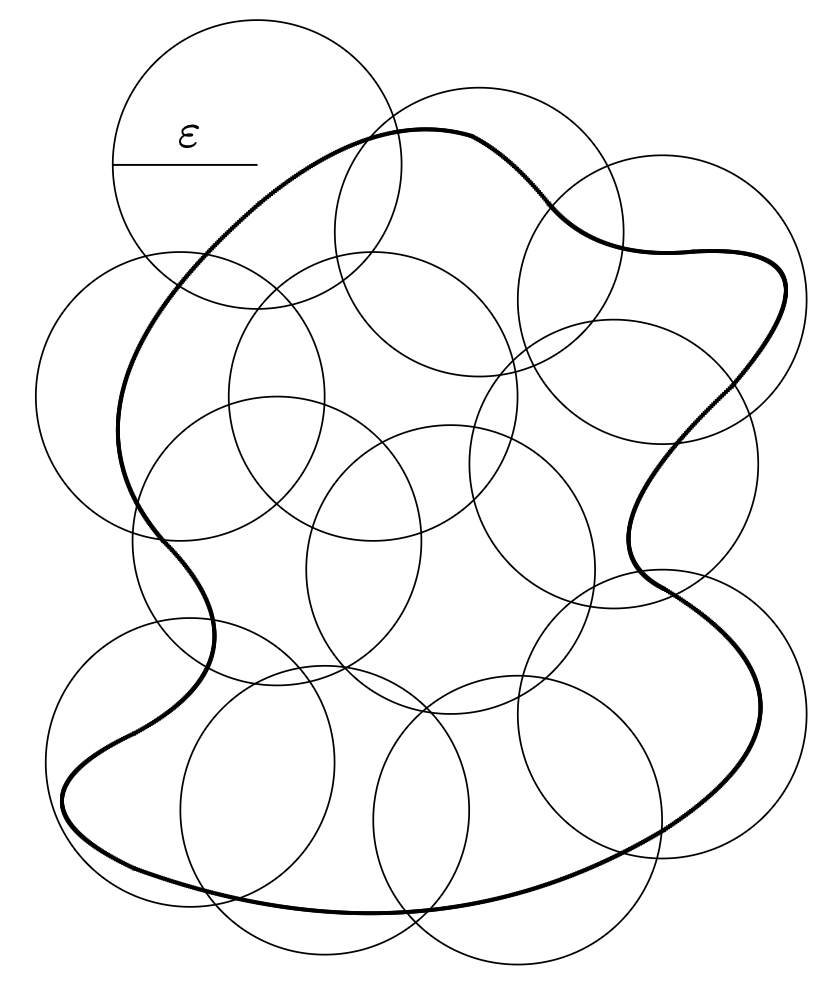
\includegraphics[width=0.5\linewidth]{pics/epsilon_cover.png}
    \caption{Example of $\epsilon$-cover. We see that $g_1, \dots, g_N$ are not necessarily in $\bG$.}
\end{figure}
%
\begin{definition}[Vector space, \href{https://ocw.mit.edu/courses/18-102-introduction-to-functional-analysis-spring-2021/8fb8d5c170f1613151aca71de21027bc_MIT18_102s21_full_lec.pdf}{Introduction to Functional Analysis}]
    A vector space $\bV$ over a field $\K$ (which we’ll take to be either $\R$ or $\C$) is a set of vectors which comes with an addition $+$: $\bV \times \bV \to \bV$ and scalar multiplication $\cdot$: $\K \times \bV \to \bV$, along with some axioms: commutativity, associativity, identity, and inverse of addition, identity of multiplication, and distributivity.
\end{definition}
%
\begin{definition}[Norm, \href{https://ocw.mit.edu/courses/18-102-introduction-to-functional-analysis-spring-2021/8fb8d5c170f1613151aca71de21027bc_MIT18_102s21_full_lec.pdf}{Introduction to Functional Analysis}]
    A norm on a \textbf{vector space} $\bV$ with field $\K$ is a function $\lVert \cdot \rVert: \bV \to [0, \infty)$ satisfying the following three properties:
    \begin{enumerate}[label=(\alph*)]
        \item (Definiteness) $\lVert v \rVert = 0$ if and only if $v = 0$.
        \item (Homogeneity) $\lVert \lambda v \rVert = |\lambda|\lVert v \rVert$ for all $v \in \bV$ and $\lambda \in \K$.
        \item (Triangle inequality) $\lVert v_1 + v_2\rVert \leq \lVert v_1\rVert + \lVert v_2\rVert$ for all $v_1, v_2 \in \bV$.
    \end{enumerate}
    A seminorm does not satisfy the first property.
\end{definition}
%
After our detour to revisit some background, let us state the assumptions made by \citet{farahmand2017value} and finally their master theorem. Consider a family of distribution $\bDelta_0$ and a \emph{pseudo-norm} $J: \bDelta \to [0, \infty]$. Let set $\bDelta_B$ used by VAML be $\bDelta_B = \left\{p \in \bDelta: J(p) \leq B \right\}$ for some $B > 0$. The reason $J$ is a pseudo-norm and not even a semi-norm is that the the set of probability distributions is not a vector space because it's not closed with respect to the addition and scalar multiplication. \citet{farahmand2017value} tried to give some examples of what $J$ could be that didn't convince me. I asked ChatGPT about possible $J$s and here are the answers:
\begin{enumerate}[label=(\Alph*)]
    \item $L_p$ norms on densities
    \item Distances between probability measures: TV, Wasserstein, KL, etc.
\end{enumerate}

\begin{assumption}[{\normalfont\citet[Assumption A1, Capacity of the function space]{farahmand2017value}}]
\label{assm:log-entrpy}
For $B >0$, let $\bDelta_B = \left\{p \in \bDelta: J(p) \leq B \right\}$. There exists constants $C > 0$ and $0 < \alpha < 1$ such that for any $\epsilon > 0$, and all sequence $z_1, \dots, z_n \in \bZ = \bS \times \bA$ the following metric entropy condition is satisfied:
\begin{equation*}
    \log \cN \left(\epsilon, \bDelta_B,  L_2(p^*_{z_{1:n}})\right) \leq C\left(\frac{B}{\epsilon}\right)^{2\alpha}.
\end{equation*}
\end{assumption}
Let the value function space be $\bV = \left\{v_\theta(s) = \phi^\top(s)\theta: \theta: \R^p, \lVert\theta\rVert_\theta \leq B \right\}$, with $\phi: \bS \to \R^p$ being the feature map.
%
\begin{theorem}[{\normalfont\citet[Theorem 2]{farahmand2017value}}]
Given a dataset $D_n = \left\{\left(S_i, A_i, S_i' \right)_{i = 1}^n \right\}$ with independent and identically distributed samples $(S_i, A_i) \sim \nu$, with $S_i' \sim p^*(\cdot \mid S_i, A_i)$, let $\hat{p}$ be the minimizer of the VAML algorithm, i.e., $\hat{p} \gets \argmin_{P \in \bDelta(\bS)} \ell^2_{2}(p, p_n^*)$, with the previously specified choice of value function space $\bV$. Let \cref{assm:log-entrpy} holds. Furthermore, assume that $\sup_{s \in \bS} \lVert \phi(s)\rVert_\infty \leq 1$ and $\sup_{s \in \bS} \lVert \phi(s)\rVert_2 \leq 1$. Fix $\delta > 0$. There exists a constant $c > 0$ such that
\begin{align}
    \text{\cref{eq:vaml-loss}} = \E \left[\sup_{v \in \bV} \left \lvert (\hat{p}_Z - p^*_Z)v\right\rvert^2 \right] \leq 
    & \underbrace{\inf_{p' \in \bDelta(\bS)}\E \left[\sup_{v \in \bV} \left\lvert (p'_Z - p^*_Z)v\right\rvert^2 \right]}_{\text{model or function approximation error}} + \\ \nonumber
    & \underbrace{c(1 + B^\alpha)p \sqrt{\frac{\log(p / \delta) }{n}} + \frac{16\log(4 /\delta)}{3n}}_{\text{estimation error}}.
\end{align}
with probability at least $1 - \delta$.
\end{theorem}
Note that since we're competing against values in $\bV$ ($\sup_{v \in \bV}$), the estimation with more data washes out and there is no residual on that part. However, since $\hat{p} \in \bDelta_B$ but we're competing against $p^* \in \bDelta$, the residual error on the model approximation persists. 

\subsection{What I didn't understand about VAML}
I just didn't go through the proofs. The arguments are clear to me.

\section{VE}
VAML exclusively studies the linear value functions case. Now, we move on to a more holistic formulation of characterizing useful models. We're going to go through all of propositions and definitions given by \citet{grimm2020value}. But, before doing so, we need to review the concept of an \emph{operator} is a functional analysis sense. 

You think simply think of an operator as a mapping (a function) from a set of functions to another set of functions. However, there is a more elegant and useful way of defining it. From linear algebra, we know that we should view functions as \emph{vectors}~\citep{strang2022introduction}. Also, from linear algebra we know that matrix-vector inner product results in a vector. So, by analogy, we are looking for an equivalent concept to matrices in infinite-dimensional spaces. Operators are the analog of matrices in functional analysis [hence their similar notation], so they turn a function into another function. Formally,
%
\begin{definition}[{\normalfont \href{https://heil.math.gatech.edu/7338/fall09/appendixc_1.pdf?utm_source=chatgpt.com}{Functional Analysis and Operator Theory}, Definition C.1}]
\label{def:operator}
Let $\bX, \bY $ be \textbf{vector spaces}, and let $T: \bX \to \bY$ be function mapping $\bX$ into $Y$. We either write $T(f)$ or $Tf$ to denote the image under $T$ of an element $f \in \bX$. Some interesting properties that involve both the function-like perspective and the matrix-like perspective.
\begin{enumerate}[label=(\Alph*)]
    \item $T$ is injective of $T(f) = T(g)$ implies $f = g$.
    \item The \emph{kernel} or \emph{null space} of if $\textsf{ker}(T) = \{f \in \bX: T(f) = 0\}$
    \item The \emph{rank} of $T$ is the is the vector space dimension of its range. In particular $T$ is finite-rank if its range is finite-dimensional.
\end{enumerate}
\end{definition}
Note that as indicated in \cref{def:operator}, the domain and the co-domain of an operator \emph{must} be vector spaces. This makes an operator different from other mappings.

We know that the Bellman equation for policy evaluation for a policy $\pi$ is written as 
\begin{equation}
    \label{eq:bllmn-evl}
    v_\pi(s) \coloneq \E_\pi \left[r^*(s, a) + \gamma \sum_{s'} p^*\left(s' \middle\vert s, a\right) v_\pi\left(s'\right)\right], \quad s \in \bS.
\end{equation}
Let us fix $\pi$ and define $r_\pi$ and $p_\pi$ as
%
\begin{equation*}
    r_\pi(s) = \sum_a \pi(a \mid s)r^*(s, a), \quad  p_\pi(\cdot \mid s) = \sum_a \pi(a \mid s) p^*(\cdot |s, a), \quad \forall s \in \bS.
\end{equation*}
Then, we can rewrite \cref{eq:bllmn-evl} as
%
\begin{equation*}
    v_\pi(s) = r_\pi(s) + \gamma \sum_{s'}p_\pi\left(s' \middle\vert s\right)v_\pi\left(s'\right), \quad \forall s \in \bS.
\end{equation*}
Now, we can define the Bellman operator for policy evaluation as
\begin{equation*}
    \left(T_\pi v\right)(s) = r_\pi(s) + \gamma \sum_{s'}p_\pi\left(s' \middle\vert s\right) v_\pi\left(s'\right), \quad \forall s \in \bS,
\end{equation*}
or by viewing $r_\pi$ as a vector in $\R^{|\bS|}$ and $p_\pi$ a matrix in $\R^{|\bS| \times |\bS|}$, compactly as $T_\pi: v \mapsto r_\pi + \gamma  p_\pi v$.
%

The Bellman optimality equation is written as 
\begin{equation}
    \label{eq:bllmn-evl}
    v^*(s) \coloneq \max_a \left\{r^*(s, a) + \gamma \sum_{s'} p^*\left(s' \middle\vert s, a\right) v^*\left(s'\right)\right\}, \quad s \in \bS.
\end{equation}
Hence, by a similar procedure for $p_\pi$, we can define the Bellman optimality operator $T^*$ as 
\begin{equation*}
    \left(T v\right)(s) = \max_a \left\{ r^*(s, a) + \gamma \sum_{s'} p^*\left(s' \middle\vert a, s\right) v^*\left(s'\right) \right\}, \quad \forall s \in \bS,
\end{equation*}
or compactly as $T: v \mapsto \max_\pi \left\{r_\pi + \gamma  p_\pi v \right\}$. Now, we have all the tools needed to dive into VE. 

Let $\bPi$ be set of all stationary Markov policies\footnote{Throughout this document, we'll only focus on stationary Markov policies, and for consciousness, we refer to them simply as policies.}, i.e., $\bPi = {\bDelta(\bA)}^{\bS} = \left\{\pi \mid \pi: \bS \to \bDelta(\bA) \right\}$, and let $\bV = \R^{\bS} = \left\{v\mid v: \bS \to \R \right\}$ be set of all value functions. Given state and action spaces, model approximation in MBRL consists an approximation of the expected immediate reward $r^*$ and an approximation of the transition kernel $p^*$. So, we if represent a model by $m = (r, p)$, where $r$ and $p$ are some arbitrary approximation, then we can represent the environment itself as the true model by $m^* = (r^*, p^*)$. Now, we can state the value equivalence principle and its associated propositions.
%
\begin{definition}[{\normalfont\citet[Definition 1]{grimm2020value}}]
\label{def:val-eqvlnc}
Let $\Pi \subseteq \bPi$ be a set of policies and let $V \subseteq \bV$ be a set of value functions. We say that two models $m$ and $\hat{m}$ are value equivalent with respect to $\Pi$ and $V$ if and only if
\begin{equation*}
    T_\pi v = \hat{T}_\pi v, \quad \forall\pi \in \Pi, \forall v \in V.
\end{equation*}
\end{definition}
\begin{quote}
    ``Two models are value equivalent with respect to $\Pi$ and $V$ if the effect of the Bellman operator induced by any policy $\pi \in \Pi$ on any function $v \in V$ is the same for both models. Thus, if we are only interested in $\Pi$ and $V$, value-equivalent models are functionally identical~\citep{grimm2020value}.''
\end{quote}
%
\begin{definition}[{\normalfont\citet{grimm2020value}[Definition 2]}]
Let $\Pi$ and $V$ be defined as in \cref{def:val-eqvlnc}. Let $M$ be a set of models. Given a model $m$, $M(\Pi, V; m)$ the set of value-equivalent models to $m$ with respect to $\Pi$ and $V$ that are in $M$, is a subset of $M$, i.e., $M(\Pi, V; m) \subseteq M$.
\end{definition}
%
Let $\bM^*$ be a set of models containing at least one model $m^*$ [I'd call it the realizable setting]. Given a set of models $M \in \bM^*$ [that doesn't necessarily contain $m^*$], often one is interested in models $m \in M$ that are value equivalent to $m^*$. We simplify the notation by defining $M^*(\Pi, V) = M(\Pi, V; m^*)$.
%
\begin{quote}
    ``The set $M^*(\Pi, V)$ contains all the models in $M$ that are value equivalent to the true model $m^*$ with respect to $\Pi$ and $V$. Since any two models $m_1, m_2 \in M^*(\Pi, V)$ are equally suitable for value-based planning using $\Pi$ and $V$, we are free to use other criteria to choose between them. For example, if $m_1$ is much simpler to represent or learn than $m_2$, it can be preferred without compromises~\citep{grimm2020value}.''
\end{quote}
%
\begin{property}[{\normalfont\citet{grimm2020value}[Property 1]}]
    \label{prpty:sbst}
    Given $M_1 \subseteq M_2$, we have that $M^*_1(\Pi, V) \subseteq M^*_2(\Pi, V)$.
\end{property}
\cref{prpty:sbst} is an elementary set topology argument. It makes sense. 
%
\begin{property}[{\normalfont\citet{grimm2020value}[Property 2]}]
    \label{prpty:m-str}
    $M^*(\bPi, \bV)$ either contains $m^*$ or is the empty set.
\end{property}
\cref{prpty:m-str} says that only the environment itself is value equivalent with respect to all policies and values. In other words, any other model that is value equivalent with respect to all policies and values is simply equivalent to the environment itself. Now, it the set of models that has been chosen $M$ doesn't contain the model of the environment, then the set of models equivalent to the environment is empty which makes sense.
%
\begin{property}[{\normalfont\citet{grimm2020value}[Property 3]}]
\label{prpty:plcy-vl-size}
Given that $\Pi_1 \subseteq \Pi_2$ and $V_1 \subseteq V_2$, we have that $M^*(\Pi_2, V_2) \subseteq M^*(\Pi_1, V_1)$.
\end{property}
Intuitively \cref{prpty:plcy-vl-size} makes sense. The bigger you make the set of policies and values you want to be equivalent to the environment, the more accurate your models should be which eventually collapses into only being the environment itself capable of achieving.  
%
\begin{property}[{\normalfont\citet{grimm2020value}[Property 4]}]
\label{prprty:m-star-in-M}
If $m^* \in M$, then $m^* \in M^*(\Pi, V)$ for all $\Pi$ and $V$.
\end{property}
\cref{prprty:m-star-in-M} is immediate from the definition of $M^*(\Pi, V)$.

\subsection{Controlling the set of equivalent models' size}
How much does $M^*(\Pi, V)$ decrease in size when we, say, add one function to V? In this section we address this and similar questions. \citet{grimm2020value} introduces the concept of $p\textsf{-span}$ which initially I found completely unnecessary given necessary definitions have already been given in functional analysis, but since $\Pi$ is not a vector space, it seems the approach of \citet{grimm2020value} is inevitable. We review the definition of $\textsf{span}$ that suffices. Also, \citet{grimm2020value} mentions \emph{discrete} sets not countable or finite. So, we must revisit what discrete means and how it is different than countable.
%
\begin{definition}[{\normalfont \citet{lax2014functional}[Theorem 2]}]
Given a vector space $\bV$ over a field $\K$, the span of set $V \subseteq \bV$ is the set of all finite linear combinations of elements $V$. Formally,
\begin{equation*}
    \textsf{span}(V) = \left\{a_1v_1 + \dots + a_nv_n \mid v_1,\dots, v_n \in V, a_1, \dots, a_n \in \K, \text{ for any } n \in \N\right\}.
\end{equation*}
\end{definition}
%
In order to understand what \emph{discrete} mean, we need to understand what: a metric space, an open set, a topology mean in order. I'll use \href{https://terrytao.wordpress.com/2009/01/30/254a-notes-8-a-quick-review-of-point-set-topology/}{this post} of Terrance Tao to understand these concepts.
\begin{definition}[Metric spaces]
    A metric space is a set $\bX$ together with a distance function $d: \bX \times \bX \to [0, \infty)$, ($\bX = (\bX, d)$) which obeys the following properties:
    \begin{enumerate}[label=(\Alph*)]
        \item (Non-degeneracy) For any $x_1, x_2 \in \bX$, we have $d(x_1, x_2) \geq 0$, with equality if and only if $x_1 = x_2$.
        \item (Symmetry) For any $x_1, x_2 \in \bX$, we have $d(x_1, x_2) = d(x_2, x_1)$.
        \item (Triangle inequality) For any $x_1, x_2, x_3 \in \bX$, we have $d(x_1, x_3) \leq d(x_1, x_2) + d(x_2, x_3)$.
    \end{enumerate}
\end{definition}
%
\begin{definition}[An open set]
    \label{def:opn-set}
    Let $(X, d)$ be a metric space. Given any $x \in \bX$ and $r > 0$, define the open ball $B(x, r)$ centered at $x$ with radius $r$ to be the set of all $y \in \bX$ such that $d(x, y) < r$. Given a set $\bE$, we say that $x$ is an interior point of $\bE$ if there is some open ball centered at $x$ which is contained in $\bE$. The set of all interior points is called the interior $\bE$.  A set is open if every point is an interior point.
\end{definition}
\cref{def:opn-set} is like our usual open interval in one dimension.
%
\begin{definition}[A topological space]
    \label{def:tplgcl-spc}
    A topological is a set $\bX$, together with a collection $\sF$ of $\bX$'s subsets, known as \emph{open sets}, which follow the following \emph{axioms}:
    \begin{enumerate}[label=(\Alph*)]
        \item $\varnothing$ and $\bX$ are open. ($\varnothing, \bX \in \sF$)
        \item The intersection of any finite number of open sets is open.
        \item The union of any arbitrary number of open sets is open.
    \end{enumerate}
    The collection $\sF$ is called a topology on $\bX$.
\end{definition}
Note that the definition of open sets in \cref{def:tplgcl-spc} is different than \cref{def:opn-set} and is by construction. So, the difference between countable and discrete is quite substantial. Countable focuses on assigning a natural number to each element, but discrete focuses of having open sets.

\paragraph{Example.} The finest (or strongest) topology on any set $\bX$ is the discrete topology $2^\bX = \{E: E \subseteq \bX\}$, in which every set is open; this is the topology generated by the discrete metric\footnote{Discrete metric $d: \bX \times \bX \to [0, \infty)$, defined by setting $d(x,y) = 0$ when $x=y$ and $d(x,y)=1$ otherwise}.  The coarsest (or weakest) topology is the trivial topology $\{\varnothing, \bX\}$, in which only the empty set and the full set are open. 

\begin{proposition}[{\normalfont\citet[Proposition 1]{grimm2020value}}]
    \label{prpstn:dscrt-pi-vl}
    For discrete [finite is correct] $\Pi$ and $V$, we have that $M^*(\Pi, V) = M^*(p\textsf{-span}(\Pi) \cap \bPi, \textsf{span}(V))$.
\end{proposition}
%
From our aforementioned definitions, it is evident that by \emph{discrete}, \citet{grimm2020value} meant \emph{finite}. Because $\Pi$ for example cannot be a discrete topology because $\{\pi_1\} \cup \{\pi_2\} = \{\pi_1, \pi_2\} \notin \Pi$. Actually, they in fact meant $\Pi$ and $V$ are finite and linearly independent, however I see no point on why limiting to this case, why not using the definition of \textsf{span} in general even for infinite-dimensional vector spaces. \cref{prpstn:dscrt-pi-vl}'s proof in the original work is correct.
%
\begin{quote}
    ``\cref{prpstn:dscrt-pi-vl} provides one possible answer to the question posed at the beginning of this section. the contraction of $M^*(\Pi, V)$ resulting from the addition of one policy to $\Pi$ or one function to $V$. For instance, if a function $v$ can be obtained as a linear combination of the functions in $V$, adding it to this set will have no effect on the space of equivalent models $M^*(\Pi, V)$~\citep{grimm2020value}.''
\end{quote}
%
Let $\bP$ be the set of all transition kernels, $P \subset \bP$ be a set of transitions, $P^*(\Pi, V)$ the set of transition kernels that are that value equivalent to $p^*$.
%
\begin{definition}[{\normalfont \citet{grimm2020value}}]
\label{def:dim}
    The dimension of a set $\bX$ is the Hamel dimension of a vector-space that encloses some translated version of $\bX$.
    \begin{equation*}
        \textsf{dim}[\bX] = \min_{\bW, \vec{c} \in W(\bX)} \textsf{H-dim}[\bW],
    \end{equation*}
    where $W(\bX) = \{(\bW, \vec{c}): \bX + \vec{c} \subseteq \bW \}$, $\bW$ is a vector space, and $\vec{c}$ is an offset.
\end{definition}
I think \cref{def:dim} is just trying to say that $\bX$ can become subspace but making sure it contains the zero vector neutralizing by $\vec{c}$.
%
\begin{remark}[{\normalfont \citet{grimm2020value}}]
    $\textsf{dim}[\bP] = (|\bS| - 1)|\bS||\bA|$.
\end{remark}
%
\begin{proof}
    By ChatGPT:
    For each $(s, a)$ the transition kernel defines a probability simplex over over $\bS$. Since the probabilities have to sum up to one there are $|\bS| - 1$ free parameters. Therefore, the total free parameters is $|\bS||\bA|(|\bS| - 1)$. \qedhere 
\end{proof}
%
\begin{proposition}[{\normalfont\citet[Proposition 2]{grimm2020value}}]
    \label{prpstn:mk-lnrly-indpndnt}
    Let $\Pi$ be set of $m$ linearly independent policies $\pi_i \in \R^{|\bS||\bA|}$ and let $V$ be the set of $k$ linearly independent vectors $v_i \in \R^{|\bS|}$, Then,
    \begin{equation*}
        \textsf{dim}[P^*(\Pi, V)] \leq |\bS|(|\bS||\bA| - mk).
    \end{equation*}
\end{proposition}
To prove \cref{prpstn:mk-lnrly-indpndnt}. We need four lemmas. I skip the first lemma as I understood what it was, though the original work had made it really convoluted. They could used an argument involving the Kronecker product instead.
%
\begin{lemma}[{\normalfont\citet[Lemma 2]{grimm2020value}}]
    For any vector $\vec{c}$ and any set $\bY + \vec{c} = \{y + \vec{c}: y \in \bY\}$, it follows that $\textsf{dim}[\bY + \vec{c}] = \textsf{dim}[\bY]$.
\end{lemma}
%
The original proof is absolutely wrong. Let's see if we can prove it ourselves.
\begin{proof}
    \begin{equation*}
        \dim[\bY + \vec{c}] = \min_{\bW, \vec{b} \in W\left(\bY + \vec{c}\right)} \Hdim [\bW].
    \end{equation*}
    Also, 
    \begin{equation*}
        W\left(\bY + \vec{c} \right) = \left\{\left(\bW, \vec{b}\right): \bY + \underbrace{\vec{c} + \vec{b}}_{\vec{d}} \in \bW\right\} = \left\{\left(\bW, \vec{b}\right): \bY + \vec{d} \in \bW\right\} = W(\bY).
    \end{equation*}
    Hence,
    \begin{equation*}
        \dim[\bY + \vec{c}] = \min_{\bW, \vec{b} \in W\left(\bY + \vec{c}\right)} \Hdim [\bW] = \min_{\bW, \vec{b} \in W\left(\bY\right)} \Hdim [\bW] = \dim[\bY].
    \end{equation*}    
\end{proof}
%
\begin{lemma}[{\normalfont\citet[Lemma 3]{grimm2020value}}]
    If $\bY$ is a vector-space, then $\Hdim[\bY] = \dim[\bY]$.
\end{lemma}
%
The original proof is correct but unnecessarily complicated. By definition,
\begin{proof}
    \begin{equation*}
        \dim[\bY] = \min_{\bW, \vec{c} \in W\left(\bY \right)} \Hdim [\bW].
    \end{equation*} 
    Since $\bY$ is a vector space and $\bW$ is also a vector space, then $\vec{c}$ must be zero (to include the the zero vector). Since $\bY$ is a vector space, it must be that $\bY = \bW$ and $\Hdim [\bW] = \Hdim[\bY]$.
\end{proof}
%
\begin{lemma}[{\normalfont\citet[Lemma 4]{grimm2020value}}]
    If $\bX \subseteq \bY$, then $\dim[\bX] \leq \dim[\bY]$.
\end{lemma}
%
The original proof is sound. The \cref{prpstn:mk-lnrly-indpndnt}'s original proof is sound except of $\min \left\{|\bS||\bA|, |\bS|m\right\} = |\bS|m$, that needs a justification that authors didn't give.
%
\begin{proposition}[{\normalfont\citet[Proposition 3]{grimm2020value}}]
    \label{prpstn:ml-is-apprxmt}
    Let $\hat{P}$ be set of approximation models. The maximum-likelihood estimate of $p^*$ in $\hat{P}$ might not belong to $\hat{P}^*(\Pi, V) \neq \varnothing$.
\end{proposition}
\cref{prpstn:ml-is-apprxmt} is saying that MLE gives an estimate that might not be useful for planning with respect to policies and values we care.
%
\begin{definition}[\href{https://www.medicine.mcgill.ca/epidemiology/hanley/bios601/Likelihood/Likelihood.pdf}{Likelihood function}]
    Let $X_1, \dots, X_n$ have a joint density function $f(X_1, \dots, X_n \mid \theta)$. Given $X_1 = x_1, \dots, X_n = x_n$ is observed, the likelihood function is defined by
    %
    \begin{equation*}
        L(\theta) = L(\theta \mid x_1, \dots, x_n) = f(x_1, \dots, x_n \mid \theta) \Big \rvert_{\text{countable setting}} = \P(x_1, \dots, x_n \mid \theta) \Big \rvert_{\text{i.i.d}} = \Pi_{i = 1}^n\P(x_i \mid \theta)
    \end{equation*}
\end{definition}
%
\begin{proof}
    I couldn't understand how the authors had computed the log-likelihood below. So, I asked ChatGPT and use its answer to make the (left out) calculation clearer. 
    
    Suppose we are trying to estimate a transition matrix $\Theta \in \R^{n \times n}$ and choose to use one parameter $\theta_i \in R$ per row. Specifically, we parametrize the distribution on the $i$-th row as
    \begin{equation*}
        \Theta_{ii} = \theta_i, \quad \theta_{ij} = \frac{1 - \theta_i}{n - 1}, \quad \text{for } j \neq j, \text{ and } \theta_i \in [0, 1]: \quad
        \Theta = \begin{pmatrix}
            \theta_1 & \frac{1 - \theta_1}{n - 1} & \dots & \frac{1 - \theta_1}{n - 1} \\
            \frac{1 - \theta_2}{n - 1} & \theta_2 & \dots & \frac{1 - \theta_2}{n - 1} \\
            \vdots & \vdots & \dots & \vdots \\
             \frac{1 - \theta_n}{n - 1} & \frac{1 - \theta_n}{n - 1} & \dots & \theta_n
        \end{pmatrix}
    \end{equation*}
    Now, we compute the \emph{expected} \emph{log}-likelihood function of $\bm{\theta} \in \R^n$. Let $N_{ij}$ denote the number of times that transition happened from $s_i$ to $s_j$ and $p_{ij}$ be the true transition probability.
    \begin{align*}
        L(\bm{\theta}) = \Pi_{i = 1}^{n}\Pi_{j = 1}^{n} \P(s_i \to s_j \mid \theta_{ij})^{N_{ij}}, \quad \text{hence} \quad \log L(\bm{\theta}) = \sum_{i = 1}^n\sum_{j = 1}^n N_{ij} \log \P(s_i \to s_j \mid \theta_{ij}).
    \end{align*}
    Since we are looking for the expected log-likelihood and $\frac{N_{ij}}{N_i} \xrightarrow{N_i \to \infty} p^*_{ij}$, we can replace the empirical frequencies with the true probability.
    \begin{equation*}
        \log L(\bm{\theta}) = \sum_{i = 1}^n\sum_{j = 1}^n p_{ij} \log \theta_{ij}
    \end{equation*}
    The maximum log-likelihood estimation $\frac{\partial\log L(\bm{\theta})}{\theta_i} = 0$ leads to $\theta_i = p^*_{ii}$. This means that the solution provided by MLE will not be exact if and only if $p_{ij} \neq p_{ik}$ for all $i \neq j \neq k$. Now, suppose we have $V = \{v\}$ with $v_i = 1$ for some $i$ and $v_j = 0$ for $j \neq i$. In this case it is possible to get an exact value-equivalent solution by making $\theta_i = p^*_{ii}$ and $\theta_j = 1 - (n -1) p^*_{ji}$ for $j \neq i$, regardless what MLE says =, which in case, since $\theta_j \neq p^*_{jj}$ is contrasting it.
\end{proof}
%
Now we have shown that MLE is not the most appropriate way of finding a value-equivalent model, \citet{grimm2020value} proposes the following objective. We ensure the imprecision of \citet{grimm2020value}'s notation is not repeated here.
%
\begin{equation*}
    \ell_{\Pi, V}(m^*, \hat{m}) = \sum_\Pi\sum_V \left\lVert Tv - \hat{T}v \right\rVert,
\end{equation*}
where $\lVert \cdot \rVert$ is a norm. Since we do not have access to $T$, we use the empirical version of it. Let $\nu \in \bDelta(\bS)$, and Let $D_\pi = \left\{\left(S_i, A_i, R_i, S'_i \right)_{i=1}^{n} \right\}$ be dataset of $n$ transitions corresponding to policy $\pi \in \Pi$, where $S_i \sim \nu(\cdot)$ and $A_i \sim \pi(\cdot \mid S_t)$. Then, the empirical value-equivalent loss is defined by
%
\begin{equation*}
    \ell_{\Pi, V, \nu}(m^*, \hat{m}) = \sum_{\pi \in \Pi}\sum_{v \in V}\sum_{s_0 \in D_\pi}\left[\left\lvert \frac{\sum_{i = 1}^{n}\II\left[S_i = s_0 \right]\left(R_i + \gamma v\left(S_i'\right) \right)}{\sum_{i = 1}^{n}\II\left[S_i = s_0 \right]} - \hat{T}v \right\rvert^p\right]^{\frac{1}{p}}.
\end{equation*}

\subsection{How to choose the subset of policies \texorpdfstring{$\Pi$}{} and values \texorpdfstring{\normalfont$V$}{}?}
\begin{proposition}[{\normalfont\citet[Proposition 4]{grimm2020value}}]
    Suppose $v \in V' \Rightarrow T_\pi v \in V'$, for all $\pi \in \Pi$. Let $\bPi \subseteq \textsf{p-span}(\Pi)$ and $\textsf{span}(V) = V'$. Then, starting form any $v' \in V'$, any $\hat{m} \in M^*(\Pi, V)$ yields the same solution as $m^*$.
\end{proposition}
The original proof is sound.

The rest of the main body of the paper is extremely ambiguous to me. I may write someday why, but I wanna move one. Honestly, I just got bored to decipher their intuitions. I'll get back to these skipped parts later.


\subsection{What I didn't understand}
\begin{enumerate}[label=(\Alph*)]
    \item Really the word \emph{discrete} in \cref{prpstn:dscrt-pi-vl}. To me they meant finite and linearly independent ad they have alluded to in the passage after Remark 1. \cref{prpstn:dscrt-pi-vl} is really suspicious.

    \item MLE in \cref{prpstn:ml-is-apprxmt} was sneaky and approximate. the counter example inside was also wrong and I changed it.

    \item Their empirical value-equivalent loss uses a wrong norm formulation.

    \item Page 6 to 9 and 17 to the end were not clear to me a t all. 
\end{enumerate}

\section{PVE}
\begin{quote}
    `` A fundamental question underlying the VE
principle is thus how to select the smallest sets of policies and functions that are sufficient for planning. In this paper we take an important step towards answering this question. We start by generalizing the concept of VE to order-$k$ counterparts defined with respect to $k$ applications of the Bellman operator. Unlike VE, the PVE class may contain multiple models even in the limit when all value functions are used. Crucially, all these models are sufficient for planning, meaning that they will yield an optimal policy despite the fact that they may ignore many aspects of the environment~\citep{grimm2021proper}.''
\end{quote}
%
PVE wants to show that only value functions are enough to specify the equivalence. Since, every policy is associated with a value function, in contrast to VE that we needed to choose $\Pi$ and $V$, now we only need to specify $\Pi$ and $V$ would naturally be their corresponding values. The main advantage of PVE over VE is that even if all value functions are considered, the class of equivalent models doesn't shrink to a singleton.

\textbf{It is crucial}: \cite{grimm2021proper} uses $T_\pi^n$ notation as the repeated application of $T_\pi$ such that $\lim_{n \to \infty} T^n_\pi v = v_\pi$.
%
\begin{definition}[Order-$k$ VE class]
    \begin{equation*}
        M_k^*(\Pi, V) = \left\{\hat{m} \in M: \hat{T}_\pi^k v = T_\pi^k v, \; \forall \pi \in \Pi, \forall v \in V \right\}.
    \end{equation*}
\end{definition}
%
\citet{grimm2021proper} claims that in contrast to \citet{grimm2020value}'s argument that $M_1^*(\bPi, \bV)$ only contains the environment, this not true for $M_k^*(\bPi, \bV)$ when $k > 1$.
%
\begin{proposition}[{\normalfont\citet[Proposition 1]{grimm2021proper}}]
    \label{prpstn:ordr-k-VE}
    Let $V$ be a set of functions such that if $v \in V$, then $T_\pi v \in V$ for all $\pi \in \Pi$. Then, for k, K in $\N$ such that $k$ divides $K$ ($k | K, \, \mathrm{or} \; K = m k, m \in \N$) , it follows that
    \begin{enumerate}[label=(\Alph*)]
        \item For any $M \subseteq \bM$ and any $\Pi \in \bPi$, we have that $M^*_k(\Pi, V) \subseteq M^*_K(\Pi, V)$.
        \item If $\Pi$ is non-empty and $V$ contains at least one constant function, then there exits environments such that $\bM^*_k(\bPi, \bV) \subset \bM^*_K(\bPi, \bV)$.
    \end{enumerate}
\end{proposition}
%
The proof the original work for \cref{prpstn:ordr-k-VE}'s part (A) is sound. For part (B), \citet{grimm2021proper} should show that all $m \in \bM^*_k(\bPi, \bV)$ are also in $\bM^*_K(\bPi, \bV)$ (which is proved by part (A)), but there exists a model $m_0 \in \bM^*_K(\bPi, \bV)$ such that $m_0 \notin \bM^*_k(\bPi, \bV)$. There is a \textbf{HUGE} subtlety for the proof of part (B) in \citet{grimm2021proper}. Specifically, they have assumed that the $k$ application of the Bellman operator $\hat{T}_\pi^k$ is the same as one application of the Bellman operator on the $k$-step return $T_\pi^{(k)}$. Using ChatGPT, now we dive into the relationship between $\hat{T}_\pi^k$ and $\hat{T}_\pi^{(k)}$.

We know that
\begin{align*}
    T_\pi v(s) & = \E_\pi \left[R_{t + 1} + \gamma v(S_{t + 1}) \middle\vert S_t = s\right], \; \text{and} \\
    G^{(k)}_t &= \E_\pi \left[R_{t + 1} + \gamma R_{t + 2} + \dots + \gamma^{k - 1} R_{t + k} + \gamma^k v(S_{t + k}) \middle\vert S_t = s\right].
\end{align*}
By induction, we'll show that
\begin{equation*}
    T^k_\pi v(s) = \E_\pi\left[\sum_{i = 0}^{k - 1} \gamma^i R_{t + i + 1} + \gamma^kv(S_{t + k}) \middle\vert S_t = s\right] = \E_\pi\left[G^{(k)}_t \middle\vert S_t = s\right].
\end{equation*}
%
\begin{proof}
\textbf{Base case}: $k = 1$ is immediate. \text{Induction step}: Suppose the the assumption for step $k$, i.e., $T^k_\pi v(s) = \E_\pi\left[\sum_{i = 0}^{k - 1} \gamma^i R_{t + i + 1} + \gamma^kv(S_{t + k}) \middle\vert S_t = s\right]$, now we show that it holds for step $k + 1$. We have
\begin{align*}
    T^{k + 1}_\pi v(s) = T_\pi\left(T^k_\pi v\right)(s) & = \E_\pi \left[R_{t + 1} + \gamma T^k_\pi v(S_{t + 1}) \middle\vert S_t = s\right] \\
    & = \E_\pi \left[R_{t + 1} + \gamma  \E_\pi\left[\sum_{i = 0}^{k - 1} \gamma^i R_{t + 1 + i + 1} + \gamma^kv(S_{t +1 + k}) \middle\vert S_{t + 1}\right] \middle\vert S_t = s\right] \\
    & = \E_\pi \left[\sum_{i = 1}^{k} \gamma^{i} R_{t + i + 1} + \gamma^{k+1} v(S_{t + 1 + k})  \middle\vert S_t = s\right]. & \tag{tower rule}
\end{align*}
\end{proof}
So, as long as the environment and the policy are deterministic (which is the case in \citet{grimm2021proper}'s proof of \cref{prpstn:ordr-k-VE}) $T^k_\pi = T^{(k)}_\pi$. With this important consideration, \citet{grimm2021proper}'s proof for part (B) is sound.
%
\begin{definition}[{\normalfont\citet[Definition 1]{grimm2021proper}}]
    \label{def:prp-ve}
    Given a set of policies $\Pi \subset \bPi$, let
    \begin{equation*}
        M_\infty^* = \lim_{k \to \infty} M_k^* (\Pi, \bV) = \{\hat{m} \in M: \hat{v}_\pi = v_\pi, \, \forall \pi \in \Pi \}.
    \end{equation*}
    We say that each $\hat{m} \in M_\infty^*$ is proper value-equivalent to the environment with respect to $\Pi$. 
\end{definition}
Since in the limit of infinite applications of the Bellman operator all value functions converge to the state-value function of a given policy, PVE only needs defining $\Pi$ in contrast to VE that needed $V$ as well.
%
\begin{proposition}[{\normalfont\citet[Definition 2]{grimm2021proper}}]
    \label{prpstn:intrsct-ve}
    For any $\Pi \in \bPi$ and $k \in \N$ it follows that
    \begin{equation*}
        M_\infty^*(\Pi) = \bigcap_{\pi \in \Pi} M_k^*(\{\pi\}, \{v_\pi\}).
    \end{equation*}
\end{proposition}
The original proof of \cref{prpstn:intrsct-ve} is sound.
%
\begin{quote}
    ``We showing how irrelevant aspects of the environment that are eventually captured by order-one VE are always ignored by PVE in \cref{prpstn:pve-ignr-irrlvnt}~\citet{grimm2021proper}.''
\end{quote}
%
\begin{proposition}[{\normalfont\citet[Proposition 3]{grimm2021proper}}]
    \label{prpstn:pve-ignr-irrlvnt}
    Let $\Pi \in \bPi$. If the environment state can be factored as $\bS = \bX \times \bY$, where $|\bY| > 1$ and $v_\pi(s) = v_\pi((x, y)) = v_\pi(x)$ for all $\pi \in \Pi$, then $\bM^*_1(\Pi, \bV) \subset \bM^*_\infty(\Pi)$.
\end{proposition}
The \cref{prpstn:pve-ignr-irrlvnt}'s original proof is okay (with some corrections in the notation and description). 
%
\begin{proposition}[{\normalfont\citet[Proposition 4]{grimm2021proper}}]
    \label{prpstn:optml-plcy}
    An optimal policy for any $\hat{m} \in M^*_\infty(\bPi)$ is an optimal policy in the environment. 
\end{proposition}
\cref{prpstn:optml-plcy} seems immediate by definition and \citet{grimm2021proper} didn't prove it either.
%
\begin{corollary}[{\normalfont\citet[Corollary 1]{grimm2021proper}}]
    \label{crllry:det-plcy-is-engh}
    Let $\bPi_\mathrm{det}$ be the set of all deterministic policies. An optimal policy for any $\hat{m} \in M_\infty^*(\bPi_\mathrm{det})$ is also optimal in the environment.
\end{corollary}
The \cref{crllry:det-plcy-is-engh}'s proof seems immediate given that one optimal policy in an MDP is deterministic~\citep{puterman2014markov}. The proof of \cref{crllry:det-plcy-is-engh} by \citet{grimm2021proper} is fine, in their proof they used the assumption of focusing on only deterministic policies that was unnecessary compared to my explanation that related it the infamous optimality of deterministic polices in \citet{puterman2014markov}.

\begin{proposition}[{\normalfont\citet[Proposition 5]{grimm2021proper}}]
    \label{prpstn:det-plcy-is-engh}
    There exits environments and model classes for which $\bM_\infty^*(\bPi) \subset M_\infty^*(\bPi_\mathrm{det})$. 
\end{proposition}
\cref{prpstn:det-plcy-is-engh}'s original proof is okay-ish.

\begin{proposition}[{\normalfont\citet[Proposition 6]{grimm2021proper}}]
    \label{prpstn:pve-dstnc}
    For any $\pi \in \bPi, v \in \bV$, and $k, n \in \N$, we have that
    \begin{equation*}
        \lVert v_\pi - \hat{T}^k_\pi v_\pi \rVert_\infty \leq (\gamma^n + \gamma^k)\lVert v_\pi - v \rVert_\infty + \lVert T^n_\pi v - \hat{T}^k_\pi v \rVert_\infty.
    \end{equation*}
\end{proposition}
\cref{prpstn:pve-dstnc}'s original proof is sound except that the authors should have made it clear that the model belongs to $M_k^*(\bPi, \bV)$.



\subsection{Promises}
\begin{enumerate}[label=(\Alph*)]
    \item Unlike VE, the PVE class \emph{may} contain multiple models even in the limit when all value functions are used. \emph{They kept it. Good job!}

    \item We construct a loss function for learning PVE models and argue that popular algorithms such as MuZero can be understood as minimizing an upper bound for this loss (with mild assumptions). \emph{Nope! The authors had confused $T^n$ and $T^(n)$ in the MuZero part.}

    \item We leverage this connection to propose a modification to MuZero and show that it can lead to improved performance in practice
\end{enumerate}

\subsection{What I didn't understand}
    \begin{enumerate}[label=(\Alph*)]
        \item On page 2 they cite Rich's and Csaba's book which were unnecessary. One of them was enough.

        \item I didn't understand the upper and lower bound on the MuZero loss. The derivation is way too sloppy.
        
    \end{enumerate}

\section{Model equivalence for risk-sensitive}
\subsection{What I didn't understand}

\section{Future work}
\begin{enumerate}[label=(\Alph*)]
    \item These papers never talked about policy search methods. What can we say about usefulness of models for those methods? In another words, if the the action space is not finite, these methods cannot explain the equivalence.

    \item These papers never talked about average reward. What can we say about usefulness of models for those methods? 
\end{enumerate}

\bibliography{my_bibs}
\end{document}
